La reconnaissance d'empreintes digitales consiste en une
reconnaissance d'un motif (empreinte sur le doigt) permettant
d'identifier le possesseur de cette empreinte. Il y a deux types
d'applications utilisant la reconnaissance d'empreintes :

\begin{description}
\item[Vérification] Une personne décline son identité et on vérifie
  que c'est vrai en comparant l'empreinte sur le doigt avec celle dans
  la base et on répond oui ou non ;
\item[Identification] On n'a aucun indice à l'avance sur l'identité du
  possesseur de l'empreinte. Il faut donc comparer l'image à toutes
  celles de la base.
\end{description}

La phase d'acquisition, généralement commune aux deux types
d'applications, correspond à l'enregistrement de l'empreinte dans la
base de donnée. Elle est généralement suivie par une algorithme de
validation de la qualité de l'enregistrement comme le montre la Figure
\ref{fig:schema-bloc-acq}.

\begin{figure}[H]
\centering
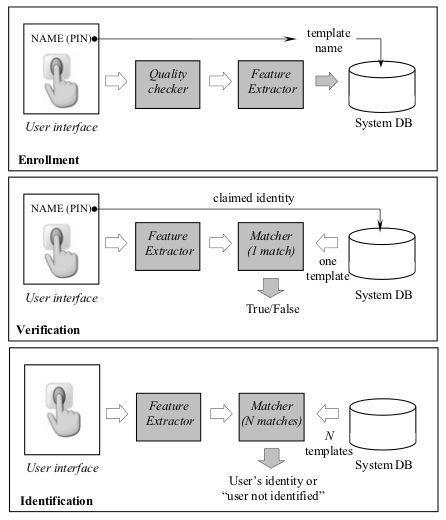
\includegraphics[scale=0.8]{three_way.png}
\caption{Schéma bloc de l'acquisition, de la vérification et de
  l'identification.}
\label{fig:schema-bloc-acq}
\end{figure}

Comme on peut le voir sur la Figure, l'image est ensuite transformée
en un modèle (\emph{template} en anglais) grâce à un extracteur de
caractéristiques (\emph{feature extractor} en anglais).

Dans le cas de la vérification, l'utilisateur entre son identifiant et
donne son empreinte. Celle-ci est transformée en un modèle compact.
On extrait le modèle lui correspondant dans la base de donnée, et un
comparateur est chargé de prendre la décision \og oui / non \fg.

Dans le cas de l'identification, c'est différent car il n'y a aucun
identifiant qui est donné et ce n'est plus un simple écart entre deux
modèles à calculer, mais un écart avec toutes les données de la base.
Les résultats possibles sont l'identité du possesseur des empreintes,
ou \og utilisateur non identifié \fg.

Il y a différentes parties distinctes, et dans un premier temps, nous
allons traiter des problèmes liés à ce type de biométrie. Dans un
second temps, nous allons traiter deux méthodes permettant la
vérification ou l'identification d'individu. La première de ces
méthodes et la méthode basé sur la corrélation entre deux empreintes
digitales. La seconde méthode se base sur les défauts que peuvent
présenter les empreintes digitales.


%%% Local Variables:
%%% mode: latex
%%% TeX-master: "../mlea"
%%% End:
